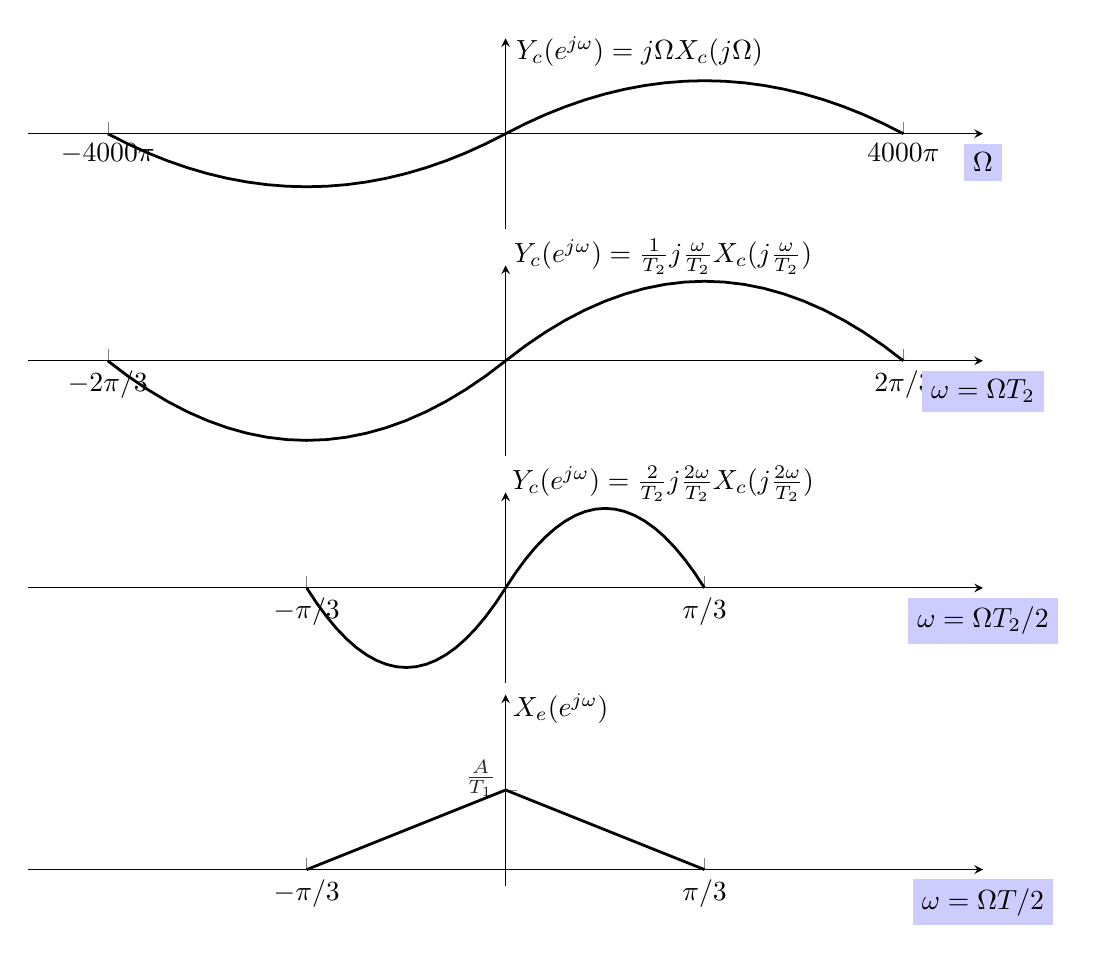
\begin{tikzpicture}
\begin{axis}[
name=plot1,
%at=(plot2.below south east), anchor=above north east,
axis lines*=middle,
enlargelimits = true,
clip=true,
scale only axis,
width=\textwidth,
height=0.2\textwidth,
ymin=-3, ymax=3,
xmin=-8, xmax=8,
axis line style={->,>=stealth},
xlabel={\tikz[baseline]{\node[fill=blue!20,anchor=base] (t1) {$\Omega$};}},
ylabel={$Y_c(e^{j\omega}) = j\Omega X_c(j\Omega)$},
every axis x label/.style={
	at={(ticklabel* cs:1)},
	%xshift=0.2cm,
	anchor=north,
},
every axis y label/.style={
	at={(ticklabel* cs:0.8)},
	anchor=south,
	xshift=1.7cm,
},
ytick=\empty,
yticklabels={$A$},
yticklabel style={yshift=0.15cm},
xtick={-8, 8},
xticklabels={$-4000\pi$, $4000\pi$}, 
every outer y axis line/.append style={white!15!black},
every y tick label/.append style={font=\color{white!15!black}},
legend style={draw=white!15!black,fill=white,legend cell align=left}]
\addplot[solid, line width=1pt, domain=-8:0, samples=21] {x*(1/8*x+1)};	
\addplot[solid, line width=1pt, domain=0:8, samples=21] {x*(-1/8*x+1)};
\end{axis}

\begin{axis}[
name=plot2,
at=(plot1.below south east), anchor=above north east,
axis lines*=middle,
enlargelimits = true,
clip=true,
scale only axis,
width=\textwidth,
height=0.2\textwidth,
%ymin=-3, ymax=3,
xmin=-8, xmax=8,
axis line style={->,>=stealth},
xlabel={\tikz[baseline]{\node[fill=blue!20,anchor=base] (t1) {$\omega = \Omega T_2$};}},
ylabel={$Y_c(e^{j\omega})  = \frac{1}{T_2}j\frac{\omega}{T_2} X_c(j\frac{\omega}{T_2})$},
every axis x label/.style={
	at={(ticklabel* cs:1)},
	%xshift=0.2cm,
	anchor=north,
},
every axis y label/.style={
	at={(ticklabel* cs:0.9)},
	anchor=south,
	xshift=2cm,
},
ytick=\empty,
yticklabels={$A$},
yticklabel style={yshift=0.15cm},
xtick={-8, 8},
xticklabels={$-2\pi/3$, $2\pi/3$}, 
every outer y axis line/.append style={white!15!black},
every y tick label/.append style={font=\color{white!15!black}},
legend style={draw=white!15!black,fill=white,legend cell align=left}]
\addplot[solid, line width=1pt, domain=-8:0, samples=21] {x*(1/8*x+1)};	
\addplot[solid, line width=1pt, domain=0:8, samples=21] {x*(-1/8*x+1)};
\end{axis}

\begin{axis}[
name=plot3,
at=(plot2.below south east), anchor=above north east,
axis lines*=middle,
enlargelimits = true,
clip=true,
scale only axis,
width=\textwidth,
height=0.2\textwidth,
%ymin=-3, ymax=3,
xmin=-16, xmax=16,
axis line style={->,>=stealth},
xlabel={\tikz[baseline]{\node[fill=blue!20,anchor=base] (t1) {$\omega = \Omega T_2/2$};}},
ylabel={$Y_c(e^{j\omega})= \frac{2}{T_2}j\frac{2\omega}{T_2} X_c(j\frac{2\omega}{T_2})$},
every axis x label/.style={
	at={(ticklabel* cs:1)},
	%xshift=0.2cm,
	anchor=north,
},
every axis y label/.style={
	at={(ticklabel* cs:0.9)},
	anchor=south,
	xshift=2cm,
},
ytick=\empty,
yticklabels={$A$},
yticklabel style={yshift=0.15cm},
xtick={-8,8},
xticklabels={$-\pi/3$, $\pi/3$}, 
every outer y axis line/.append style={white!15!black},
every y tick label/.append style={font=\color{white!15!black}},
legend style={draw=white!15!black,fill=white,legend cell align=left}]
\addplot[solid, line width=1pt, domain=-8:0, samples=21] {x*(1/8*x+1)};	
\addplot[solid, line width=1pt, domain=0:8, samples=21] {x*(-1/8*x+1)};
\end{axis}

\begin{axis}[
name=plot4,
at=(plot3.below south east), anchor=above north east,
axis lines*=middle,
enlargelimits = true,
clip=true,
scale only axis,
width=\textwidth,
height=0.2\textwidth,
ymin=0, ymax=2,
xmin=-16, xmax=16,
axis line style={->,>=stealth},
xlabel={\tikz[baseline]{\node[fill=blue!20,anchor=base] (t1) {$\omega =\Omega T/2$};}},
ylabel={$X_e(e^{j\omega})$},
every axis x label/.style={
	at={(ticklabel* cs:1)},
	%xshift=0.2cm,
	anchor=north,
},
every axis y label/.style={
	at={(ticklabel* cs:0.8)},
	anchor=south,
	xshift=0.7cm,
},
ytick={1},
yticklabels={$\frac{A}{T_1}$},
yticklabel style={yshift=0.15cm},
xtick={-8, 8},
xticklabels={$-\pi/3$, $\pi/3$}, 
every outer y axis line/.append style={white!15!black},
every y tick label/.append style={font=\color{white!15!black}},
legend style={draw=white!15!black,fill=white,legend cell align=left}]
\addplot[solid, line width=1pt] coordinates {(-8, 0) (0, 1) (8, 0)};	
%\addplot[solid, line width=1pt] coordinates {(-6, 0) (-6, 1/4) (-2, 3/4) (-2, 0) (2, 0) (2, 3/4) (6, 1/4) (6, 0)};	
\end{axis}

\end{tikzpicture}
